\documentclass[handout,compress]{beamer}

\usetheme[block=fill]{metropolis}

\usepackage{graphicx} % Allows including images
\usepackage{amsmath,amsfonts,amsthm,amssymb}
\usepackage{color}
\usepackage{xcolor,cancel}
%\setitemize{label=\usebeamerfont*{itemize item}%
%	\usebeamercolor[fg]{itemize item}
%	\usebeamertemplate{itemize item}}
\definecolor{mDarkBrown}{HTML}{604c38}
\definecolor{mDarkTeal}{HTML}{23373b}
\definecolor{mLightBrown}{HTML}{EB811B}
\definecolor{mMediumBrown}{HTML}{C87A2F}
\definecolor{mygreen}{HTML}{98C2B9}
\definecolor{myyellow}{HTML}{DFD79C}
\definecolor{myblue}{HTML}{8CA7CC}
\definecolor{kern}{HTML}{8CC2B7}

\usepackage{float}
\usepackage{framed}
\usepackage{epsfig}
\usepackage{graphicx}
\usepackage{subcaption}
\usepackage{ulem}
\usepackage{hhline}
\usepackage{multirow}
\usepackage{comment}   
\usepackage{bbm}
\usepackage{tikz}   
\usepackage{ulem}
\def\Put(#1,#2)#3{\leavevmode\makebox(0,0){\put(#1,#2){#3}}}
\newcommand*\mystrut[1]{\vrule width0pt height0pt depth#1\relax}
\newcommand{\eqdef}{\mathbin{\stackrel{\rm def}{=}}}


\newcommand{\bs}[1]{\boldsymbol{#1}}
\newcommand{\bv}[1]{\mathbf{#1}}
\newcommand{\R}{\mathbb{R}}
\newcommand{\E}{\mathbb{E}}

\DeclareMathOperator*{\argmin}{arg\,min}
\DeclareMathOperator*{\argmax}{arg\,max}
\DeclareMathOperator{\nnz}{nnz}
\DeclareMathOperator{\Var}{Var}
\DeclareMathOperator{\sinc}{sinc}
\DeclareMathOperator{\mv}{mv}
\DeclareMathOperator{\sgn}{sgn}
\DeclareMathOperator{\step}{step}
\DeclareMathOperator{\gap}{gap}
\DeclareMathOperator{\poly}{poly}
\DeclareMathOperator{\tr}{tr}
\DeclareMathOperator{\orth}{orth}
\newcommand{\norm}[1]{\|#1\|}
\captionsetup[subfigure]{labelformat=empty}
\captionsetup[figure]{labelformat=empty}
\DeclareMathOperator*{\lmin}{\lambda_{min}}
\DeclareMathOperator*{\lmax}{\lambda_{max}}

\newcommand{\specialcell}[2][c]{%
  \begin{tabular}[#1]{@{}c@{}}#2\end{tabular}}
\newcommand{\specialcellleft}[2][c]{%
\begin{tabular}[#1]{@{}l@{}}#2\end{tabular}
}

\usepackage{tabstackengine}
\stackMath

\newtheorem{claim}[theorem]{Claim}


%----------------------------------------------------------------------------------------
%	TITLE PAGE
%----------------------------------------------------------------------------------------

\title{CS-UY 4563: Lecture 13 \\ Kernel Methods}
\author{NYU Tandon School of Engineering, Prof. Christopher Musco}
\date{}

\begin{document}

\begin{frame}
	\titlepage 
\end{frame}

\metroset{titleformat=smallcaps}

\begin{frame}
	\frametitle{course admin}
	\textbf{My new office:} \url{https://nyu.zoom.us/my/cmusco}
	\begin{itemize}
		\item Visit this URL during my office hours or any individual meetings.
		\item You can also ``drop in" even if I'm not in the chat. I will receive an email notification (might take me a few minutes to notice) and can then let you in if I'm free.
		\item For lectures still use the links on NYU Classes (which allows for automatic recording, transcription, etc.)
	\end{itemize}
\end{frame}

\begin{frame}
		\frametitle{course project}
			\textbf{By 4/1 (next Wednesday)  choose a partner and topic.}

			\begin{itemize}
				\item Email me team members, project topic, and a sentence or two about your idea. If you have any data sets in mind, let me know that as well.
				\item Then set up a meeting at: \footnotesize{\url{https://docs.google.com/spreadsheets/d/1DsR7ia4VfYb5joIavsG8_T1JBgAufkVbdT7bLfPGGQ0/edit?usp=sharing}}.
			\end{itemize}
\end{frame}


\begin{frame}
	\frametitle{lets ease back into things}
	\textbf{$k$-NN algorithm:} a simple but powerful baseline for classification.
	
	\textbf{Training data:} $(\vec{x}_1, y_1), \ldots, (\vec{x}_n, y_n)$ where $y_1, \ldots, y_n \in \{1,\ldots, q\}$. 
	
	\textbf{Classification algorithm:}
	
	Given new input $\vec{x}_{new}$,
	\begin{itemize}
		\item Compute $sim(\vec{x}_{new}, \vec{x}_1), \ldots, sim(\vec{x}_{new}, \vec{x}_n).$
		\item Let $\vec{x}_{j_1}, \ldots, \vec{x}_{j_k}$ be the $k$ training data vectors with highest similarity to $\vec{x}_{new}$. 
		\item Predict $y_{new}$ as $majority(y_{j_1}, \ldots, y_{j_k})$.
	\end{itemize}
\end{frame}

\begin{frame}
	\frametitle{inner product similarity}
	Given data vectors $\vec{x},\vec{w}\in \R^d$, the inner product $\langle\vec{x}, \vec{w}\rangle$ is a natural similarity measure.
	\begin{align*}
	\langle\vec{x}, \vec{w}\rangle = \sum_{i=1}^d \vec{x}[i]\vec{w}[i] = \cos(\theta)\|\vec{x}\|_2\|\vec{w}\|_2.
	\end{align*}
		\begin{center}
		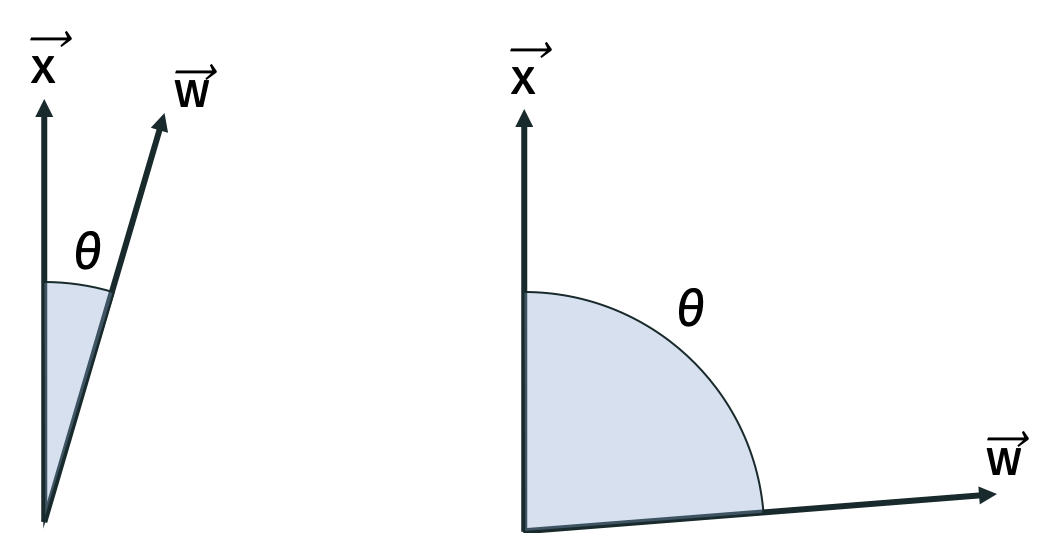
\includegraphics[width=.7\textwidth]{inner_product_similarity.png}
	\end{center}
\end{frame}

\begin{frame}
	\frametitle{mnist image data}
	Each pixel is number from $[0,1]$. $0$ is black, $1$ is white. 
	Represent $28\times 28$ matrix of pixel values as a flattened vector.
	\begin{center}
		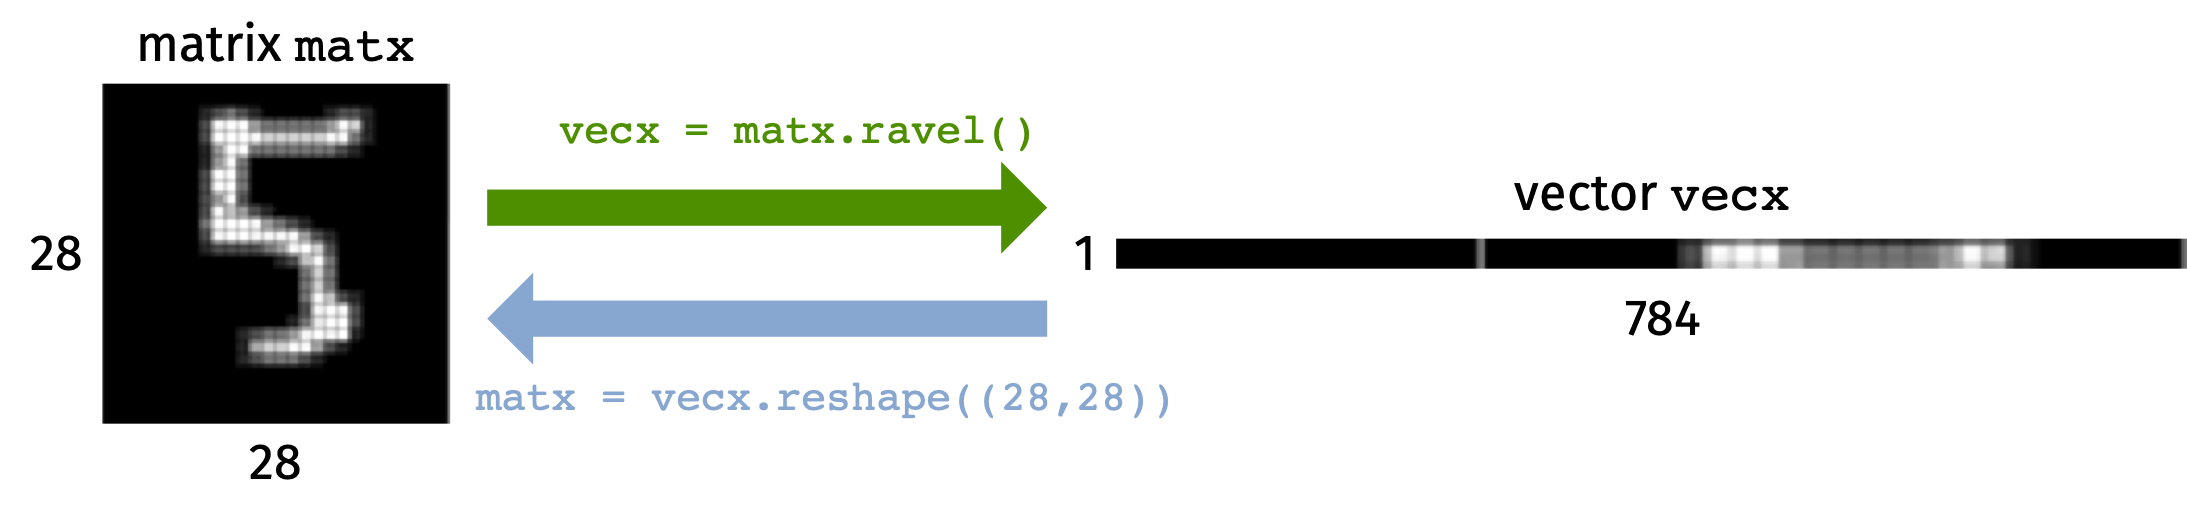
\includegraphics[width=\textwidth]{flatten.png}
		
		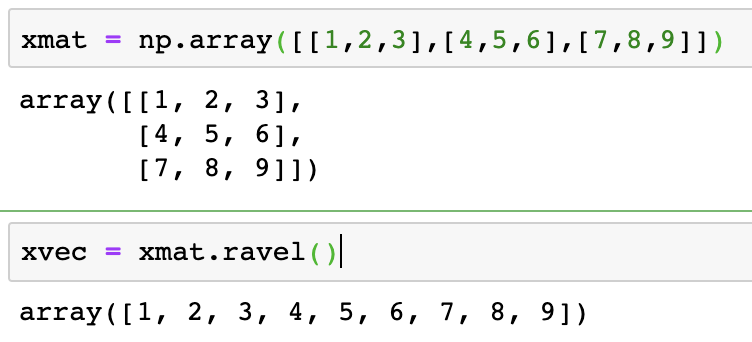
\includegraphics[width=.7\textwidth]{flatten_code.png}
	\end{center}
\end{frame}

\begin{frame}
	\frametitle{inner product for mnist}
	Inner product between MNIST digits:
	\begin{center}
			
\includegraphics[width=.8\textwidth]{flat_compare.png}
	\begin{align*}
	\langle \vec{x},\vec{w}\rangle = \sum_{i=1}^{28} \sum_{j=1}^{28} \texttt{matx}[i,j]\texttt{matw}[i,j].
	\end{align*}
	\end{center}
	Inner product similarity is higher when the images have large pixel values (close to $1$) in the same locations. I.e. when they have a lot of overlapping white/light gray pixels.
\end{frame}

\begin{frame}
	\frametitle{inner product for mnist}
	\textbf{Visualizing the inner product between two images:}
		\begin{center}
			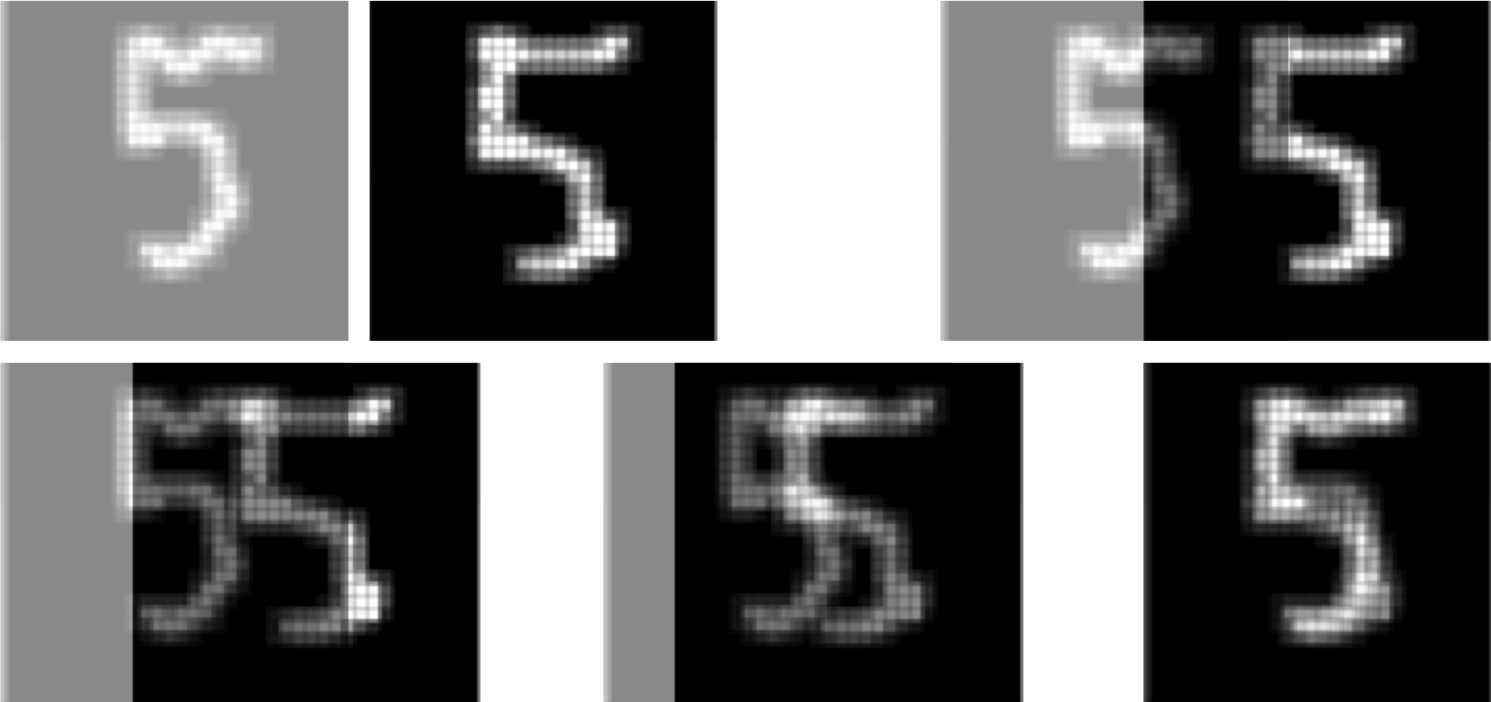
\includegraphics[width=.8\textwidth]{innerproduct_visualizatoin.png}
		\end{center}
	Images with high inner product have a lot of overlap.
\end{frame}

\begin{frame}
	\frametitle{view of logistic regression}
	\textbf{One-vs.-all Classification with Logistic Regression:}
	\begin{itemize}
		\item Learn $q$ classifiers with parameters $\vec{\beta}_0, \vec{\beta}_1, \ldots, \vec{\beta}_{q-1}$.
		\item Given $\vec{x}_{new}$ compute $\langle \vec{x}_{new}, \vec{\beta}_0\rangle, \ldots, \langle\vec{x}_{new}, \vec{\beta}_{q-1}\rangle$
		\item Predict class $y_{new} = \argmax_i \langle\vec{x}_{new}, \vec{\beta}_i\rangle$.
	\end{itemize}
	If each $\vec{x}$ is a vector with $28\times 28 = 784$ entries than each $\vec{\beta}_i$ also has $784$ entries. Each parameter vector can be viewed as a $28\times 28$ image. 
\end{frame}

\begin{frame}
	\frametitle{matched filter}
	Visualizing $\vec{\beta}_0, \ldots, \vec{\beta}_{9}$:
	\begin{center}
		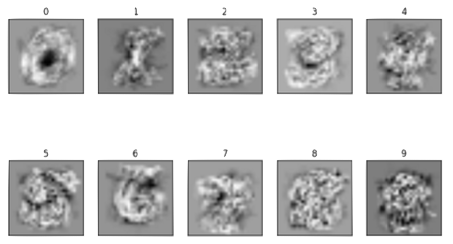
\includegraphics[width=.7\textwidth]{logweights.png}
	\end{center}
For an input image \hspace{.5em}
\includegraphics[width=.05\textwidth]{five.png}\hspace{.5em}, compute \emph{inner product} similarity with all weight matrices and choose most similar one. 

In contrast to $k$-NN, only need to compute similarity with $q$ items instead of $n$.
\end{frame}

\begin{frame}
	\frametitle{view of logistic regression}
	\begin{center}
		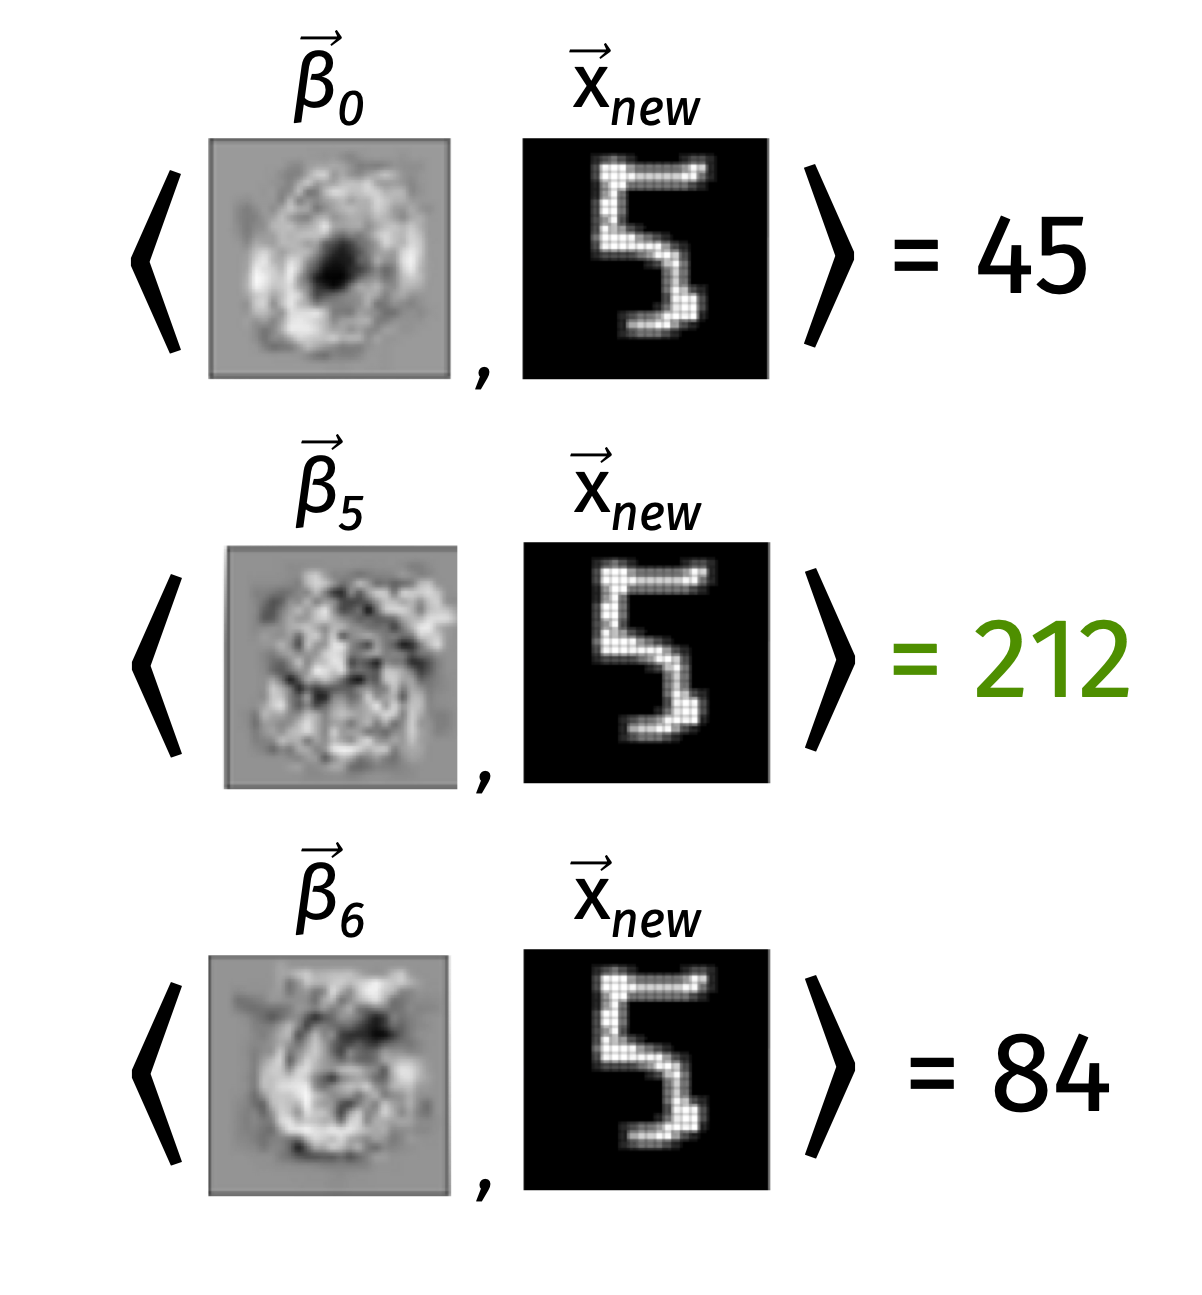
\includegraphics[width=.5\textwidth]{orig_form.png}
		
		Select class for $\vec{x}_{new}$ which achieves highest ``score'', as measured by the inner product similarity.
	\end{center}
\end{frame}

\begin{frame} 
	\frametitle{alternative view}
	\textbf{Logistic Regression Model:}
	
	Given data matrix $\bv{X} \in \R^{n\times d}$ (here $d = 784$) and binary label vector $\vec{y}\in \{0,1\}^n$ for class $i$ (1 if in class $i$, 0 if not), find $\vec{\beta}_i \in \R^d$ to minimize the log loss between:
	\begin{align*}
	&\vec{y} & &\text{and} & h(\bv{X}\vec{\beta})
	\end{align*}
	where $h(\bv{X}\vec{\beta}_i) = \frac{1}{1 + e^{-\bv{X}\vec{\beta}_i}}$ applies the logistic function entrywise to the vector $\bv{X}\vec{\beta}$.
	
	
	Loss = $-\sum_{j=1}^n y_j\log(h(\bv{X}\vec{\beta}_i)[j]) +  (1-y_j)\log(1- h(\bv{X}\vec{\beta}_i)[j])$
	
\end{frame}

\begin{frame} 
	\frametitle{alternative view}
		\textbf{Logistic Regression Model:}
	
	Given data matrix $\bv{X} \in \R^{n\times d}$ (here $d = 784$) and binary label vector $\vec{y}\in \{0,1\}^n$ for class $i$ (1 if in class $i$, 0 if not), find $\vec{\beta} \in \R^d$ to minimize the log loss between:
	\begin{align*}
	&\vec{y} & &\text{and} & h(\bv{X}\vec{\beta})
	\end{align*}
	
		
	\textbf{Reminder from linear algebra:}
	Without loss of generality, can assume that $\vec{\beta}$ lies in the \emph{row span} of $\bv{X}$. 
	
	So for any $\vec{\beta} \in \R^d$, there exists a vector $\vec{\alpha}\in \R^n$ such that:
	\begin{align*}
	\vec{\beta} = \bv{X}^T \vec{\alpha}.
	\end{align*}
	
\end{frame}

\begin{frame} 
	\frametitle{alternative view}
	\textbf{Logistic Regression Equivalent Formulation:}
	
	Given data matrix $\bv{X} \in \R^{n\times d}$ (here $d = 784$) and binary label vector $\vec{y}\in \{0,1\}^n$ for class $i$ (1 if in class $i$, 0 if not), \alert{\emph{find $\vec{\alpha} \in \R^n$}} to minimize the log loss between:
	\begin{align*}
	&\vec{y} & &\text{and} & h(\bv{X}\bv{X}^T\vec{\alpha}).
	\end{align*}
	
	Can still be minimized via gradient descent:
	\begin{align*}
		\nabla L(\vec{\alpha}) = \bv{X}\bv{X}^T(h(\bv{X}\bv{X}^T\vec{\alpha}) - \vec{y}).
	\end{align*}
	
\end{frame}

\begin{frame} 
	\frametitle{reformulated view}
	What does classification for a new point $\vec{x}_{new}$ look like? Recall that for a given one-vs-all classification $i$, the original parameter vector $\vec{\beta}_i = \bv{X}^T\vec{\alpha}_i$.
	
	\begin{itemize}
	\item Learn $q$ classifiers with parameters $\vec{\alpha}_1, \vec{\alpha}_2, \ldots, \vec{\alpha}_q$.
	\item Given $\vec{x}_{new}$ compute $\langle \vec{x}_{new}, \bv{X}^T\vec{\alpha}_1\rangle, \ldots, \langle\vec{x}_{new}, \bv{X}^T\vec{\alpha}_q\rangle$
	\item Predict class $y_{new} = \argmax_i \langle\vec{x}_{new}, \bv{X}^T\vec{\alpha}_i\rangle$.
\end{itemize}
	
\end{frame}

\begin{frame} 
	\frametitle{reformulated view}
	\textbf{Score for class $i$:}
	\begin{align*}
	\langle\vec{x}_{new}, \bv{X}^T\vec{\alpha}_i\rangle &=\vec{x}_{new}^T \bv{X}^T\vec{\alpha}_i \\
	&= \langle\bv{X}\vec{x}_{new}, \vec{\alpha}_i\rangle \\
	&= \sum_{j=1}^n \vec{\alpha}_i[j] \langle\vec{x}_{new}, \vec{x}_j\rangle.
	\end{align*}
%	Similar to $k-NN$ classifier but we learn a \emph{weight} $\alpha_i$ for every $\vec{x}_i$ in our training set -- can be positive or negative. 
%	
\end{frame}

\begin{frame}
	\frametitle{original view of logistic regression}
	\begin{center}
		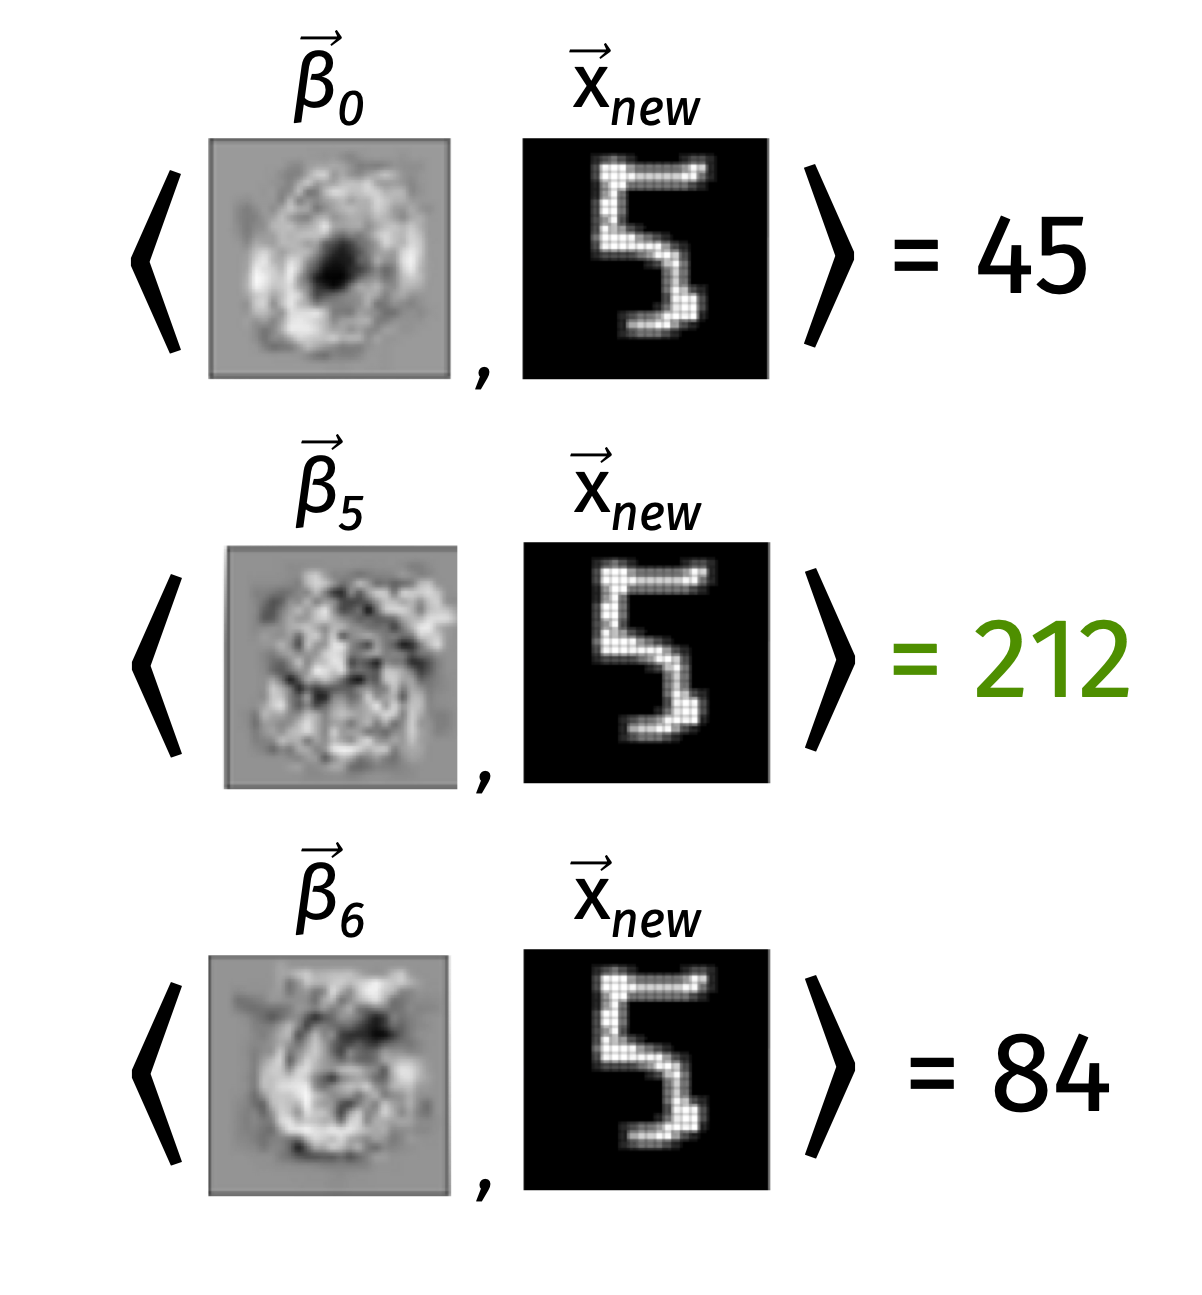
\includegraphics[width=.5\textwidth]{orig_form.png}
	\end{center}
\end{frame}

\begin{frame}
	\frametitle{new view of logistic regression}
	\begin{center}
		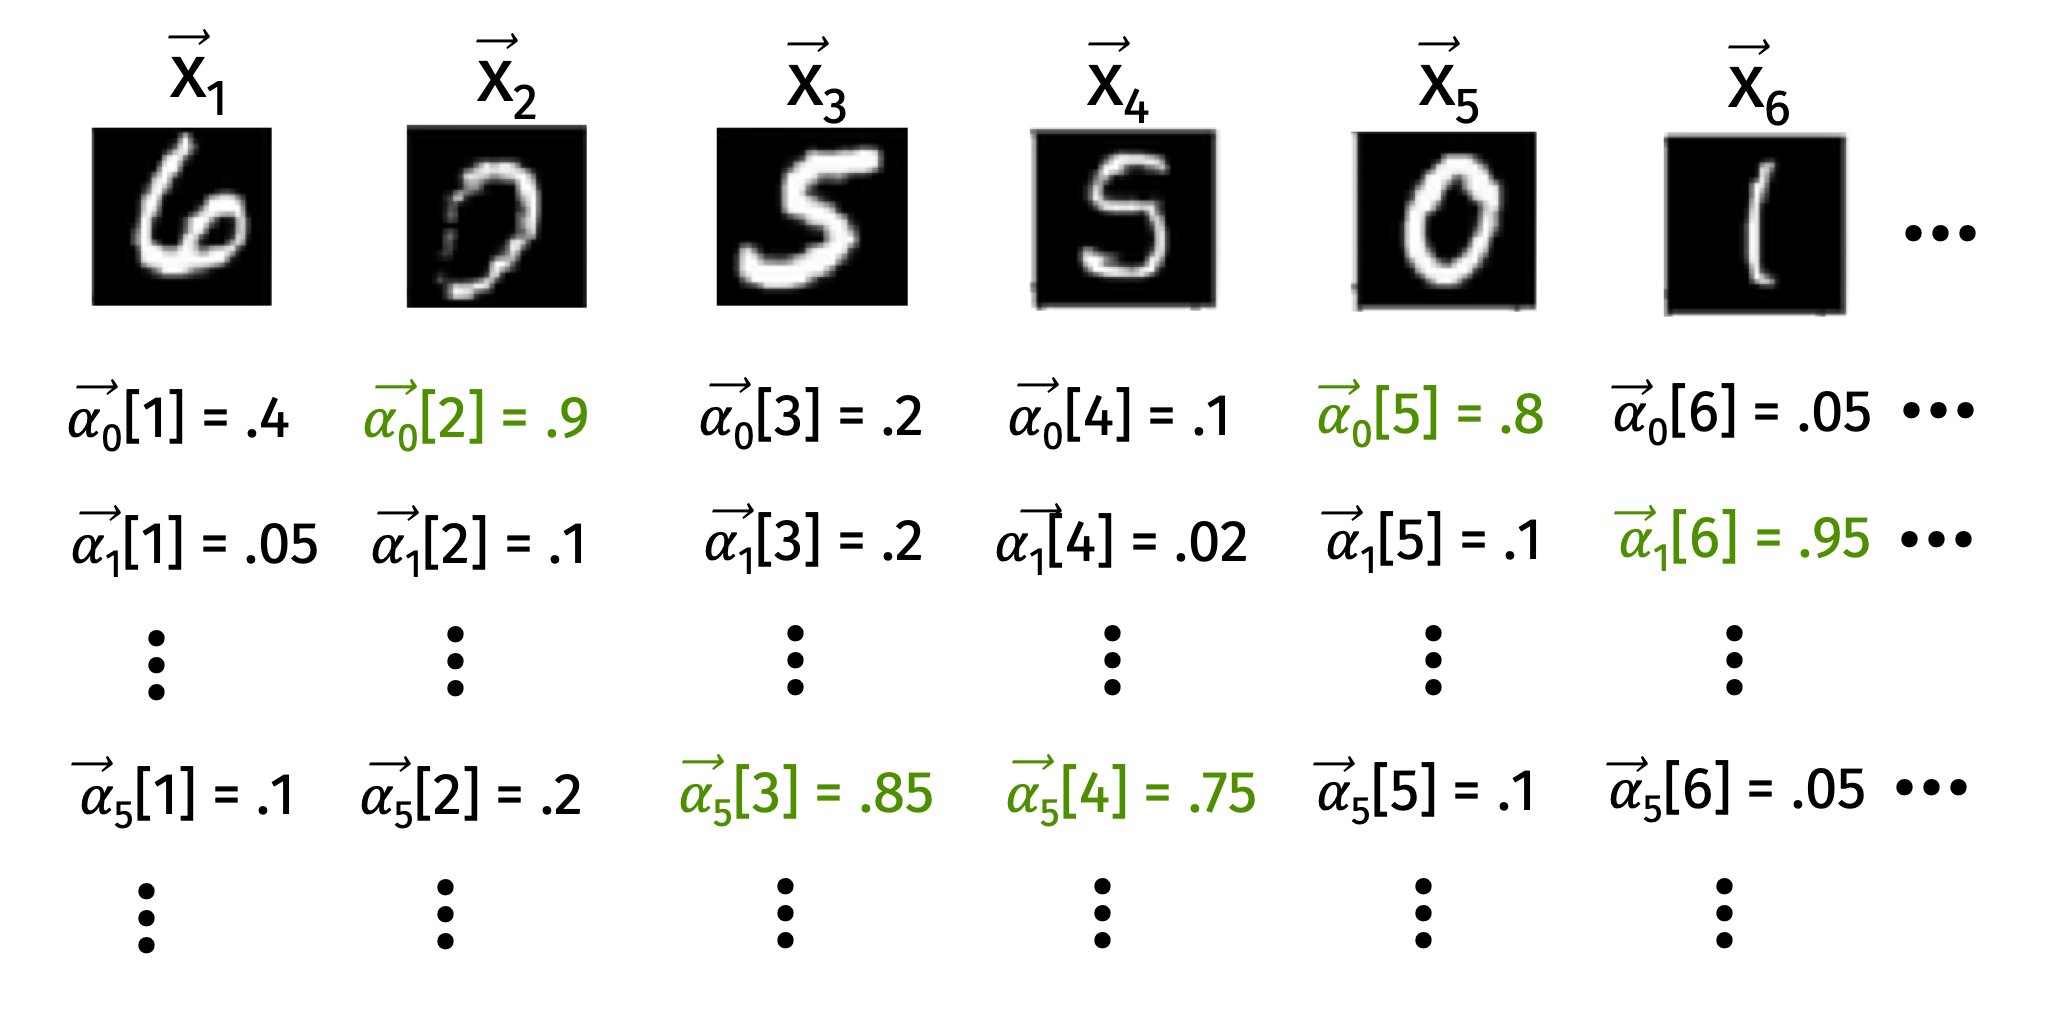
\includegraphics[width=\textwidth]{scores.png}
		
		Learn $n$ length parameter vectors $\vec{\alpha}_0,\ldots, \vec{\alpha}_{9}$, one for each class.
	\end{center}
\end{frame}

\begin{frame}
	\frametitle{new view of logistic regression}
	\begin{center}
		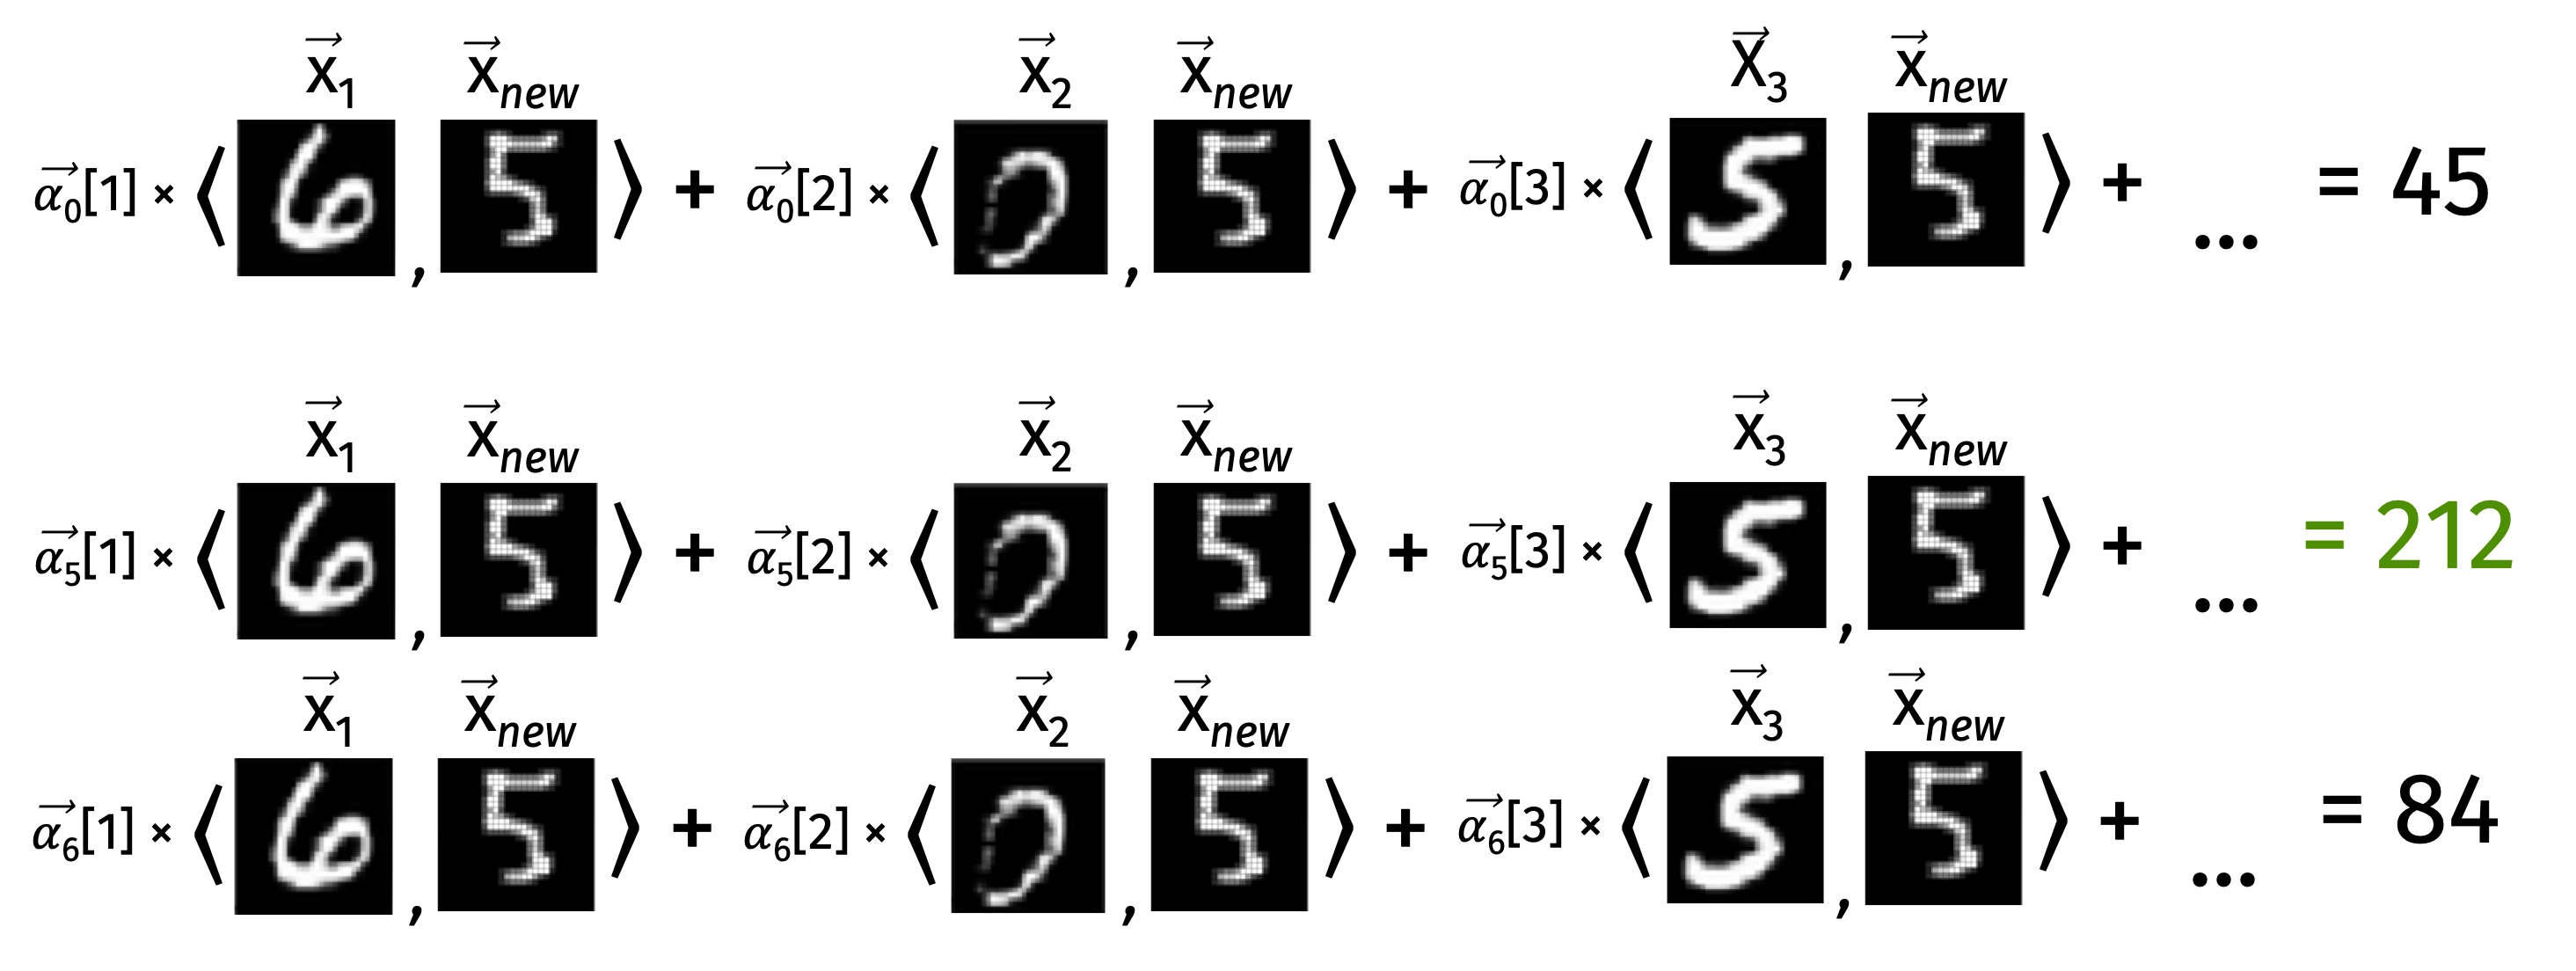
\includegraphics[width=\textwidth]{new_form.png}
		
		Classification looks similar to $k$-NN: we compute the \emph{similarity} between $\vec{x}_{new}$ and every other vector in our training data set. A weighted sum of the similarities leads to scores for each class. 
	\end{center}
Assign $\vec{x}_{new}$ to the class with highest score. 
\end{frame}


\begin{frame}
	\frametitle{diving into similarity}
	Often the inner product \alert{does not make sense} as a \emph{similarity} measure between data vectors. Here's an example (recall that smaller inner product means less similar):
	\begin{center}
		
\includegraphics[width=.7\textwidth]{bad_inner_product.png}
		
		But clearly the first image is more similar. 
		
		
		
\includegraphics[width=.7\textwidth]{better_inner_product.png}
		
		Here's a more realistic scenario.
	\end{center}
\end{frame}


\begin{frame} 
	\frametitle{kernel functions: perspective one}
	A \emph{kernel function} $k(\vec{x}, \vec{y})$ is simply a similarity measure between data points. 
	\begin{align*}
	k(\vec{x}, \vec{y}) = \begin{cases}
		\text{large if $\vec{x}$ and $\vec{y}$ are similar.}\\
		\text{close to $0$ if $\vec{x}$ and $\vec{y}$ are different.}
	\end{cases}
	\end{align*}
	\textbf{Example:} The Radial Basis Function (RBF) kernel, aka the Gaussian kernel:
	\begin{align*}
		k(\vec{x}, \vec{y}) = e^{-\|\vec{x} - \vec{y}\|_2^2/\sigma^2}
	\end{align*}
	for some scaling factor $\sigma$. 
	\begin{center}
	
\includegraphics[width=.7\textwidth]{rbf_similarity.png}
	\end{center}
\end{frame}

\begin{frame}
	\frametitle{kernel functions: perspective one}
	Lots of kernel functions functions involve transformations of $\langle \vec{x},\vec{y}\rangle$ or $\|\vec{x} - \vec{y}\|_2$:
	\begin{itemize}
		\item Gaussian RBF Kernel: $k(\vec{x}, \vec{y}) = e^{-\|\vec{x} - \vec{y}\|_2^2/\sigma^2}$
		\item Laplace Kernel: $k(\vec{x}, \vec{y}) = e^{-\|\vec{x} - \vec{y}\|_2/\sigma}$
		\item Polynomial Kernel: $k(\vec{x}, \vec{y}) = (\langle \vec{x},\vec{y}\rangle + 1)^q$.
	\end{itemize}
But you can imagine much more complex similarity metrics. 
\end{frame}

\begin{frame} 
	\frametitle{kernel functions: perspective two}
	For a simple algorithm like $k$-NN you can swap our the inner product similarity with \emph{any similarity function you could possibly imagine}. 
	
	For a methods like logistic regression, this is not the case... 
	
	\textbf{Recall:} We learned a parameter vector $\vec{\alpha}$ to minimize $LL(\vec{y}, \bv{X}^T\vec{\alpha})$ where $LL()$ denotes the logistic loss. Then we classified via:
	\begin{align*}
	\langle\vec{x}_{new}, \bv{X}^T\vec{\alpha}\rangle =\vec{x}_{new}^T \bv{X}^T\vec{\alpha} 
	= \sum_{j=1}^n \vec{\alpha}[j] \langle\vec{x}_{new}, \vec{x}_j\rangle.
	\end{align*}
	The \emph{inner product} similarity came from the fact that our predictions were based on the \emph{linear function} $\bv{X}^T \alpha$.	
\end{frame}

\begin{frame} 
	\frametitle{kernel functions as feature transformation}
	A \emph{positive semidefinite} (PSD) kernel is any similarity function with the following form:
	\begin{align*}
	k(\vec{x},\vec{w}) = \phi(\vec{x})^T \phi(\vec{w})
	\end{align*}
	where $\phi: \R^d \rightarrow \R^m$ is a some feature transformation function. 
\end{frame}

\begin{frame} 
	\frametitle{kernel functions and feature transformation}
	\small
	\textbf{Example:} Degree 2 polynomial kernel, $k(\vec{x},\vec{w}) = (\vec{x}^T\vec{w} + 1)^2$.
	\begin{align*}
	\vec{x} &= \begin{bmatrix}x_1\\x_2\\x_3\end{bmatrix} & \phi(\vec{x}) &= \begin{bmatrix}1\\ \sqrt{2}x_1\\\sqrt{2}x_2\\\sqrt{2}x_3 \\ x_1^2 \\ x_2^2 \\ x_3^2 \\ \sqrt{2}x_1x_2 \\ \sqrt{2}x_1x_3 \\ \sqrt{2}x_2x_3\end{bmatrix}  
	\end{align*}
	\begin{align*}
	(\vec{x}^T\vec{w} + 1)^2 &= ({x}_1{y}_1 + {x}_2{y}_2  + {x}_3{y}_3  + 1)^2\\
	&=  1 + 2{x}_1{w}_1 + 2{x}_2{w}_2 + 2{x}_3{w}_3 +  {x}_1^2{w}_1^2 + {x}_2^2{w}_2^2  + {x}_3^2{w}_3^2 \\ & \hspace{1em} + 2{x}_1{w}_1{x}_2{w}_2  +2{x}_1{w}_1{x}_3{w}_3 +2{x}_2{w}_2{x}_3{w}_3\\
	&= \phi(\vec{x})^T\phi(\vec{w}).
	\end{align*}
\end{frame}

\begin{frame} 
	\frametitle{kernel functions and feature transformation}
	Not all similarity metrics you are positive semidefinite (PSD), but all of the ones we saw earlier are:
	\begin{itemize}
		\item Gaussian RBF Kernel: $k(\vec{x}, \vec{y}) = e^{-\|\vec{x} - \vec{y}\|_2^2/\sigma^2}$
		\item Laplace Kernel: $k(\vec{x}, \vec{y}) = e^{-\|\vec{x} - \vec{y}\|_2/\sigma}$
		\item Polynomial Kernel: $k(\vec{x}, \vec{y}) = (\langle \vec{x},\vec{y}\rangle + 1)^q$.
	\end{itemize}
	And there are many more...
\end{frame}

\begin{frame} 
	\frametitle{kernel functions and feature transformation}
	\begin{center}
		\textbf{Feature transformations $\Longleftrightarrow$ new similarity metrics.}
	\end{center}
	Using $k(\cdot,\cdot)$ in place of the inner product $\langle\cdot,\cdot\rangle$ is \textbf{\alert{equivalent}} to replacing every data point $\vec{x}_1,\ldots, \vec{x}_n$ in our data set with $\phi(\vec{x}_1), \ldots, \phi(\vec{x}_n)$. 
	\begin{center}
		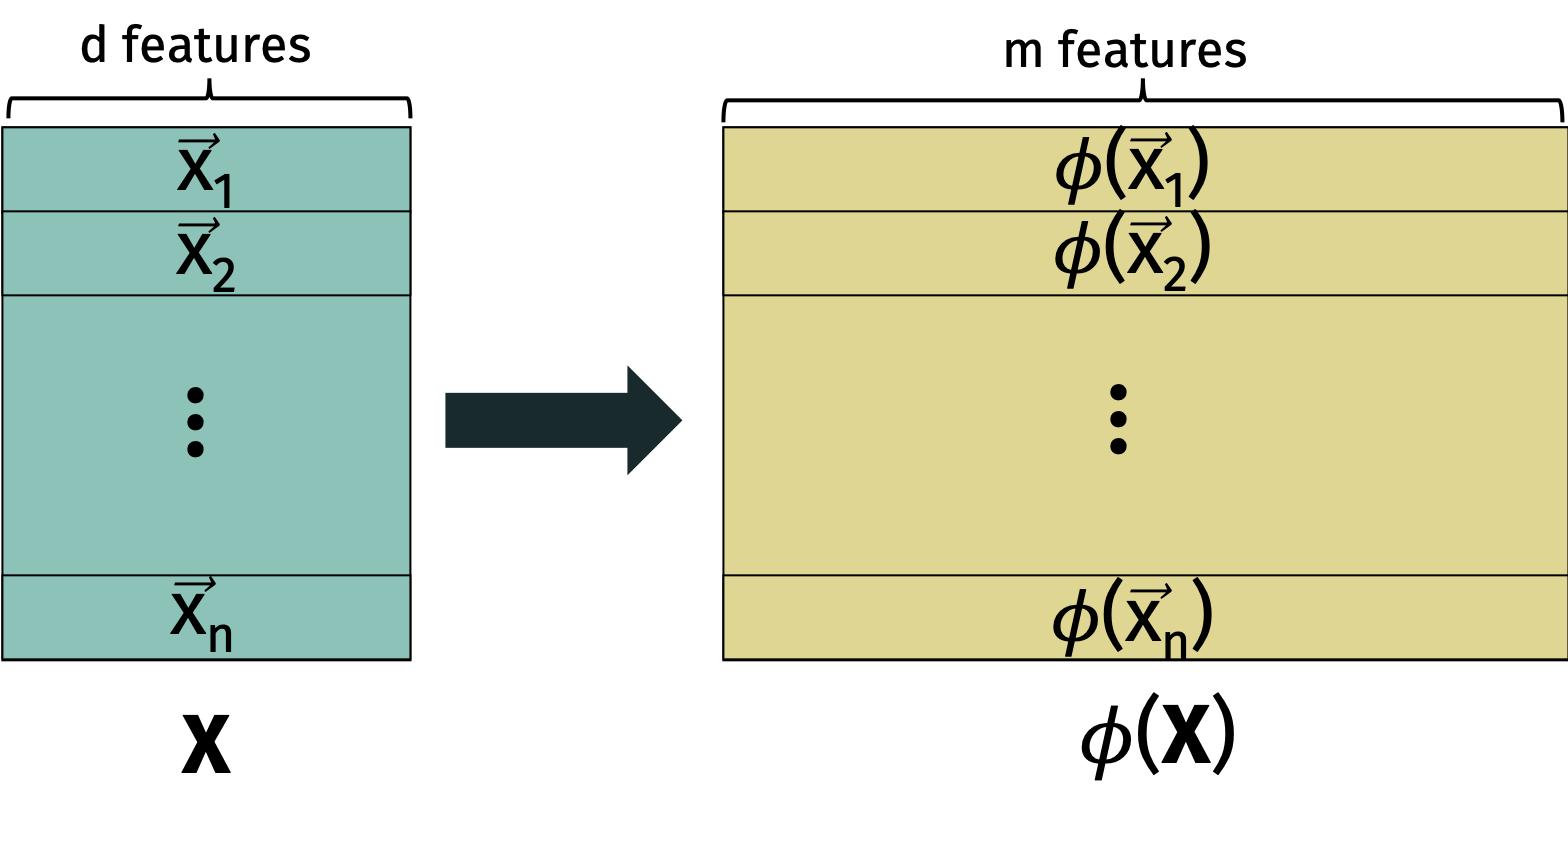
\includegraphics[width=.7\textwidth]{feature_transformation.png}
	\end{center}
\end{frame}

\begin{frame} 
	\frametitle{takeaway one}
	We can improve performance by replacing the inner product with another kernel $k(\cdot,\cdot)$ for the same reason that feature transformations improved performance.
	\begin{center}
		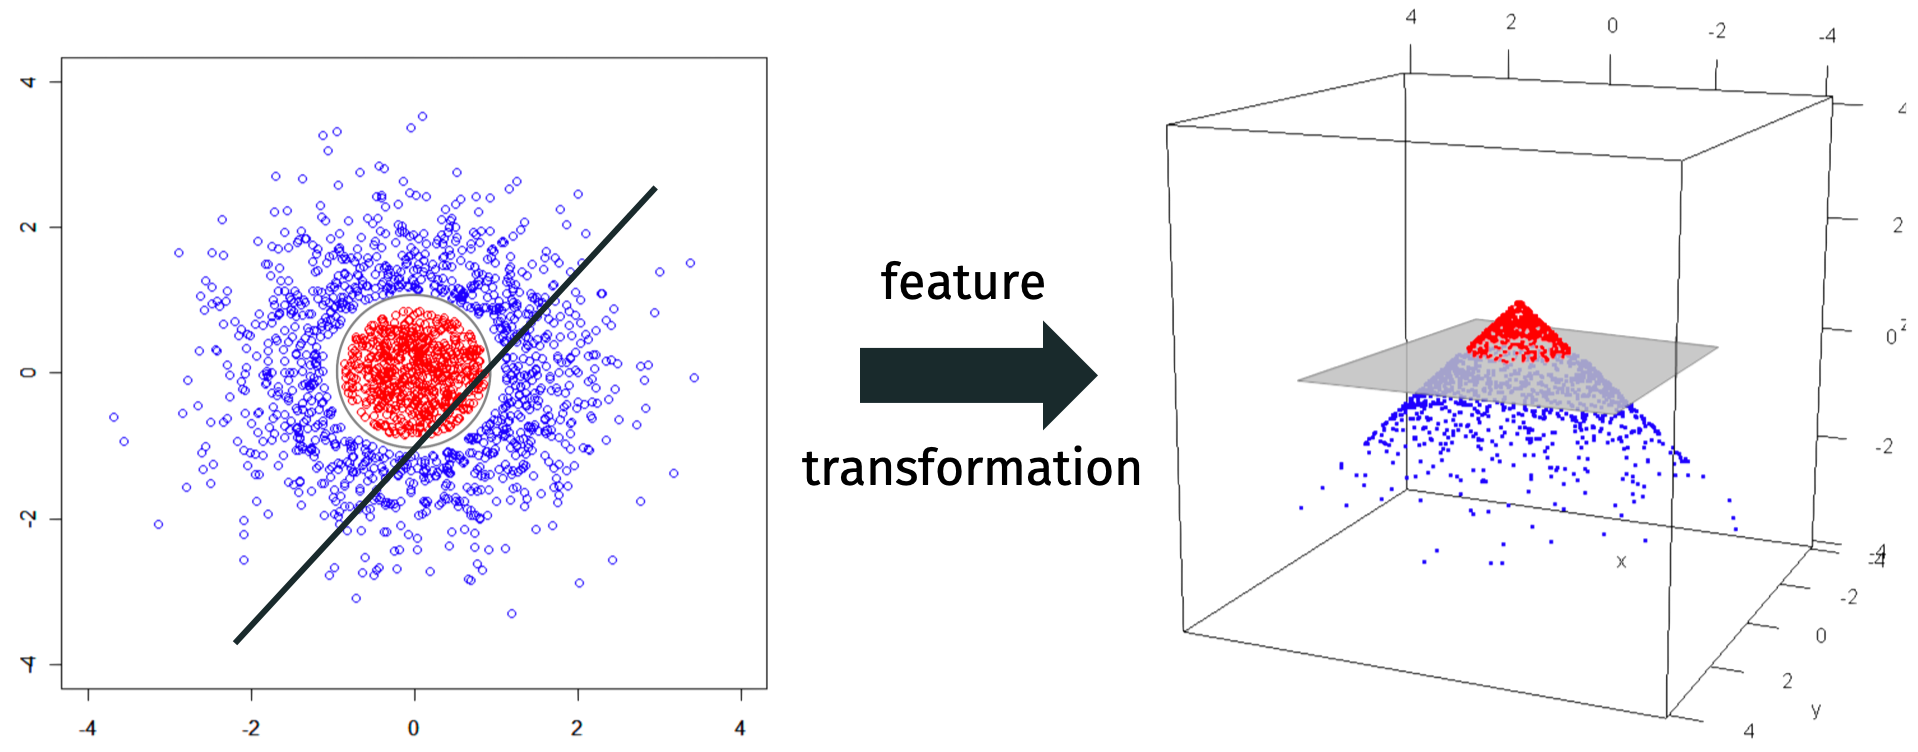
\includegraphics[width=.8\textwidth]{kernel_vis.png}
	\end{center}
	When you add features, it becomes possible to learn more complex decision boundaries (in this case a circle) with a linear classifier.
\end{frame}

\begin{frame} 
	\frametitle{takeaway two}
	PSD kernel functions give a principled way of ``swapping out'' the inner product with a new similarity metric for linear algorithms like multiple linear regression or logistic regression.
	
For non-PSD kernels it is not clear how to do this.
\end{frame}


\begin{frame} 
	\frametitle{kernel logistic regression}
	\begin{columns}[t]
		\begin{column}{.5\textwidth}
			\emph{\textbf{Standard logisitic regression}}
			\vspace{1em}
			
			Loss function: 
			\begin{align*}
			L(\vec{\alpha}) = LL(\vec{y}, \bv{X}^T\vec{\alpha}).
			\end{align*}
			
			
			Gradient:
			\begin{align*}
			\nabla L(\vec{\alpha}) = \bv{X}\bv{X}^T(h(\bv{X}\bv{X}^T\vec{\alpha}) - \vec{y}).
			\end{align*}
			
			Prediction:
			\begin{align*}
			z &= \sum_{j=1}^n \vec{\alpha}[j] \langle\vec{x}_{new}, \vec{x}_j\rangle.\\
			y_{new} &= \mathbbm{1}[z > 0]
			\end{align*}
		\end{column}
		\begin{column}{.5\textwidth}
			\emph{\textbf{Kernel logisitic regression}}
			\vspace{1em}
			
			Loss function: 
			\begin{align*}
			L(\vec{\alpha}) = LL(\vec{y}, \phi(\bv{X})^T\vec{\alpha}).
			\end{align*}
			
			
			Gradient:
			\begin{align*}
			\nabla L(\vec{\alpha}) = \phi(\bv{X})\phi(\bv{X})^T(h(\phi(\bv{X})\phi(\bv{X})^T\vec{\alpha}) - \vec{y}).
			\end{align*}
			
			Prediction:
			\begin{align*}
			z &= \sum_{j=1}^n \vec{\alpha}[j] \langle\phi(\vec{x}_{new}), \phi(\vec{x}_j)\rangle \\
			y_{new} &= \mathbbm{1}[z > 0]
			\end{align*}
		\end{column}
	\end{columns}
\end{frame}

\begin{frame} 
	\frametitle{kernel regression}
	\begin{columns}[t]
		\begin{column}{.5\textwidth}
			\emph{\textbf{Standard linear regression}}
			\vspace{1em}
			
			Loss function: 
			\begin{align*}
			L(\vec{\alpha}) = \|\vec{y}- \bv{X}\bv{X}^T\vec{\alpha}\|_2
			\end{align*}
			
			
			Gradient:
			\begin{align*}
			\nabla L(\vec{\alpha}) = 2\bv{X}\bv{X}^T(\bv{X}\bv{X}^T\alpha- \vec{y}).
			\end{align*}
			
			Prediction:
			\begin{align*}
			y_{new}  = \sum_{j=1}^n \vec{\alpha}[j] \langle\vec{x}_{new}, \vec{x}_j\rangle.
			\end{align*}
		\end{column}
		\begin{column}{.5\textwidth}
		\emph{\textbf{Kernel linear regression}}
		\vspace{1em}
	
		Loss function: 
		\begin{align*}
		L(\vec{\alpha}) = \|\vec{y}- \phi(\bv{X})\phi(\bv{X})^T\vec{\alpha}\|_2
		\end{align*}
	
	
		Gradient:
		\begin{align*}
		\nabla L(\vec{\alpha}) = 2\phi(\bv{X})\phi(\bv{X})^T(\phi(\bv{X})\phi(\bv{X})^T\alpha- \vec{y}).
		\end{align*}
	
		Prediction:
		\begin{align*}
		y_{new}  = \sum_{j=1}^n \vec{\alpha}[j] \langle\phi(\vec{x}_{new}), \phi(\vec{x}_j)\rangle.
		\end{align*}
	\end{column}
	\end{columns}
\end{frame}

\begin{frame}
	\frametitle{kernel regression}
	We won't study kernel \emph{regression} in detail, but it's a very important statistical tool, especially when dealing with spatial or temporal data.
	\begin{center}
		\includegraphics[width=.5\textwidth]{gp_regression.png}\includegraphics[width=.4\textwidth]{kriging.png}
	\end{center}
Also known as Gaussian Process (GP) Regression or Kriging. 
\end{frame}

\begin{frame} 
	\frametitle{kernel matrix}
	\begin{center}
	$\bv{K} = \phi(\bv{X})\phi(\bv{X})^T$ is called the \emph{kernel Gram matrix}.
	
	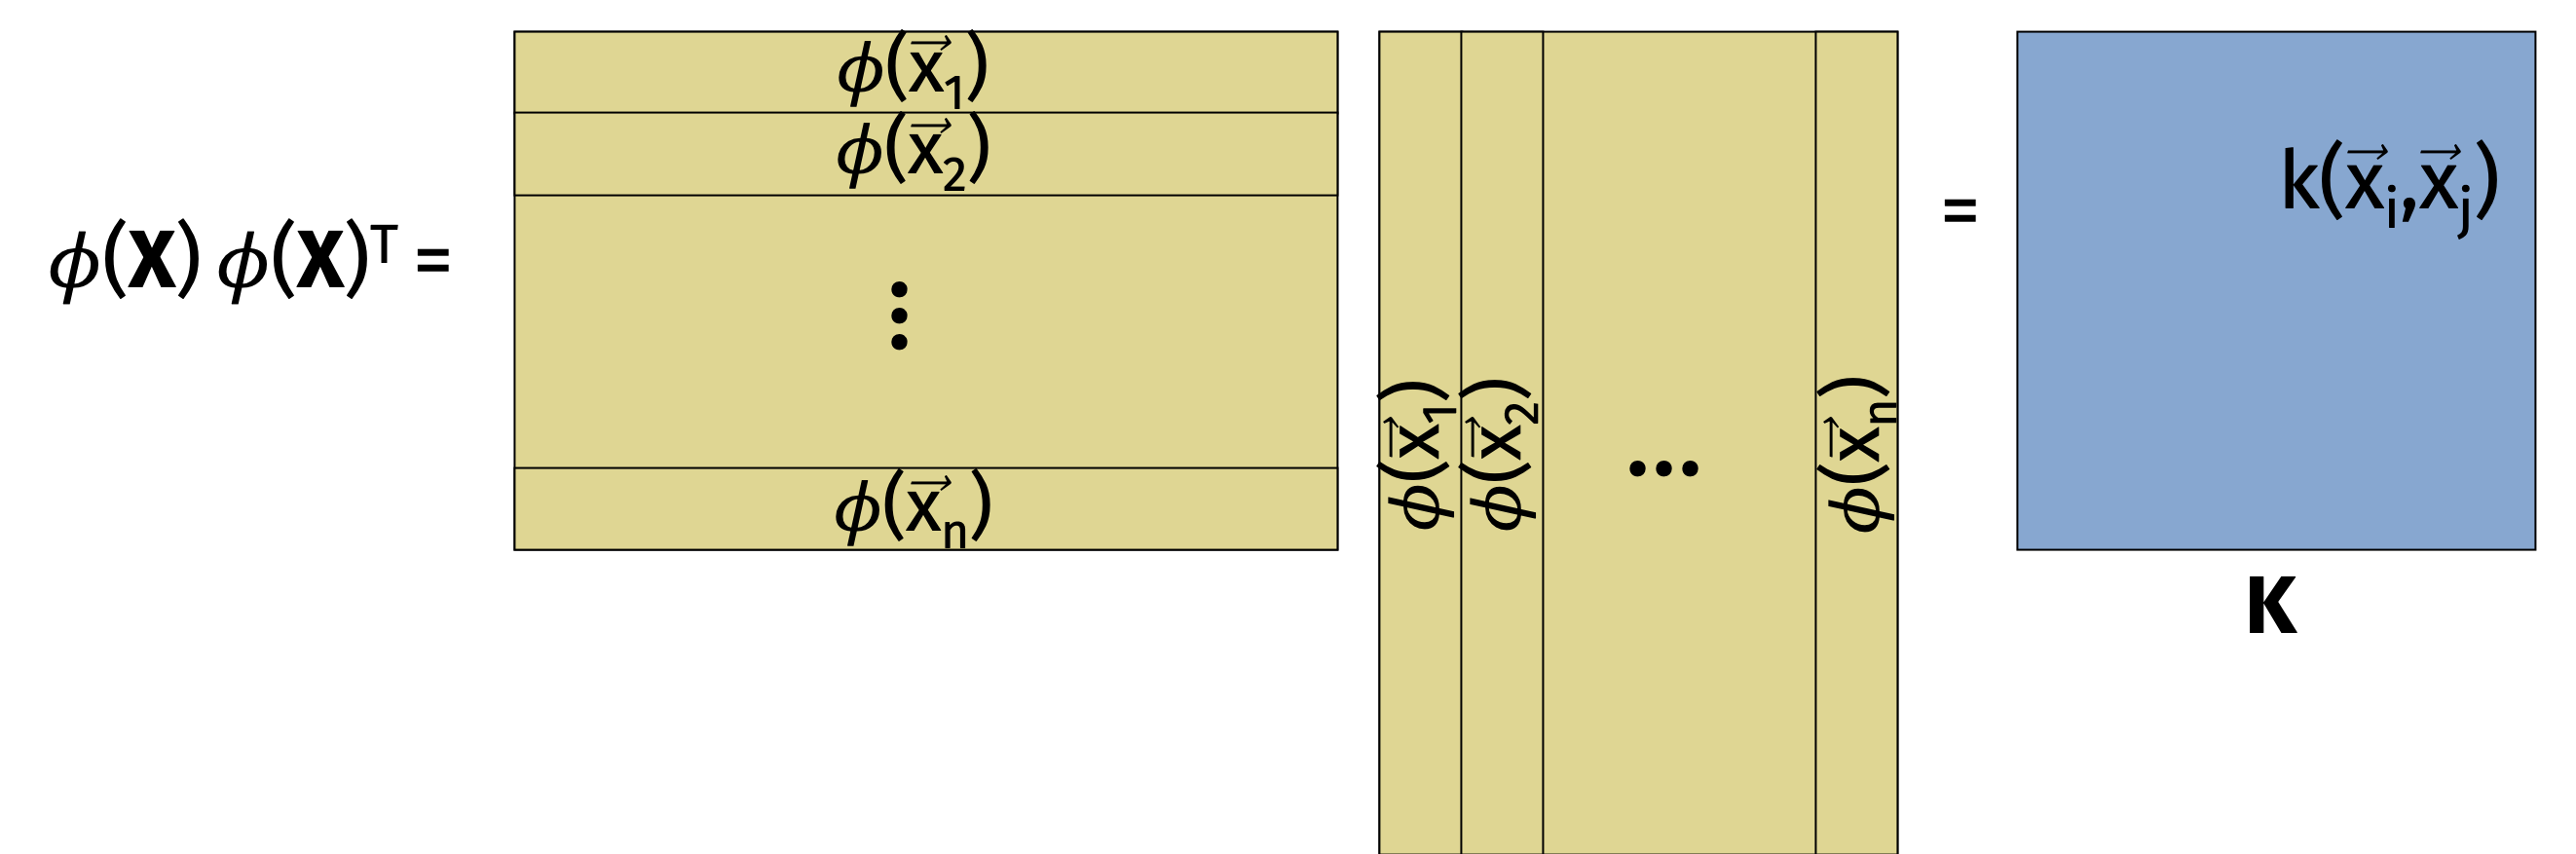
\includegraphics[width=\textwidth]{kernel_matrix.png}
	\end{center}
\end{frame}

\begin{frame} 
	\frametitle{kernel trick}
	We never need to actually compute $\phi(\vec{x}_1), \ldots, \phi(\vec{x}_n)$ explicitly: 
	\begin{itemize}
		\item For training we just need the kernel matrix $\bv{K}$, which requires computing $k(\vec{x}_i,\vec{x}_j)$ for all $i,j$. 
		\item For testing we just need to compute $k(\vec{x}_{new},\vec{x}_i)$ for all $i$. 
	\end{itemize}
\begin{center}
	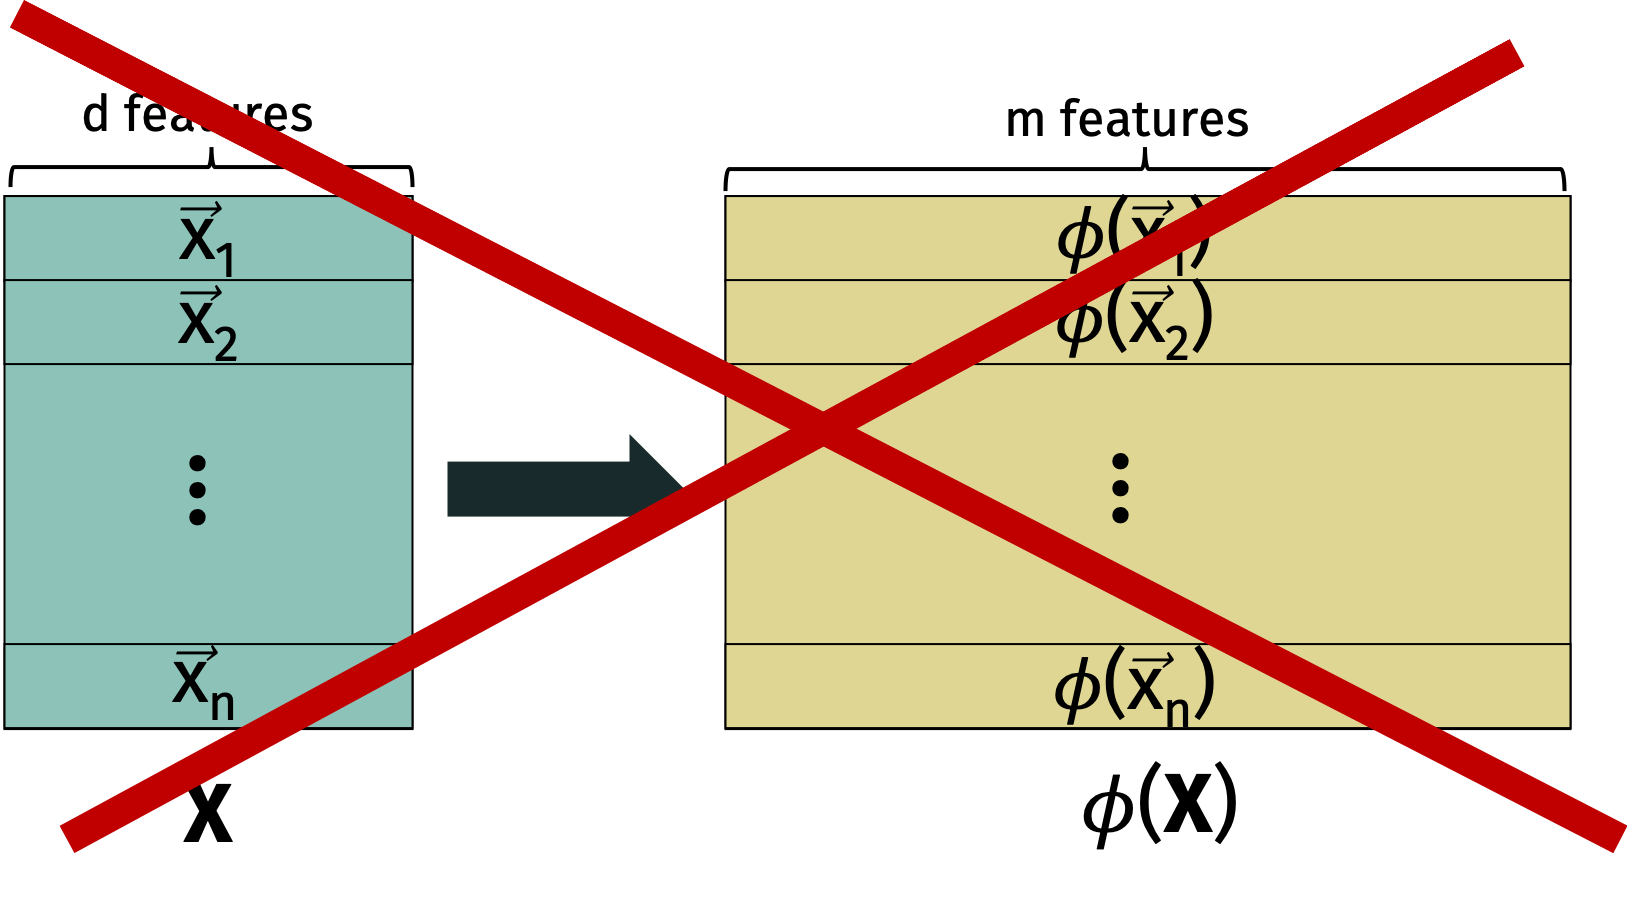
\includegraphics[width=.8\textwidth]{kernel_adv.png}
\end{center}
\end{frame}

\begin{frame} 
	\frametitle{kernel trick}
	This can lead to significant computational savings!
	\begin{itemize}
		\item Transform dimension $m$ is often very large: e.g. $m = O(d^q)$ for a degree $q$ polynomial kernel. 
		\item For many kernels (e.g. the Gaussian kernel) $m$ is actually \textit{infinite}. 
	\end{itemize}
\end{frame}

\begin{frame} 
	\frametitle{beyond the kernel trick}
	The kernel matrix $\bv{K}$ is still $n \times n$ though which is huge when the number of data examples $n$ is large. Has made the kernel trick less appealing in some modern ML applications.
	
	Many algorithmic advances in recent years partially address this computational challenge (random Fourier features methods, Nystrom methods, etc.)
	
\end{frame}

\end{document} 






